\documentclass{standalone}
\usepackage{tikz}
\usepackage{xcolor}

\usetikzlibrary{decorations.pathmorphing}
\usetikzlibrary{shapes}
\usetikzlibrary{shapes.geometric}

\begin{document}
	
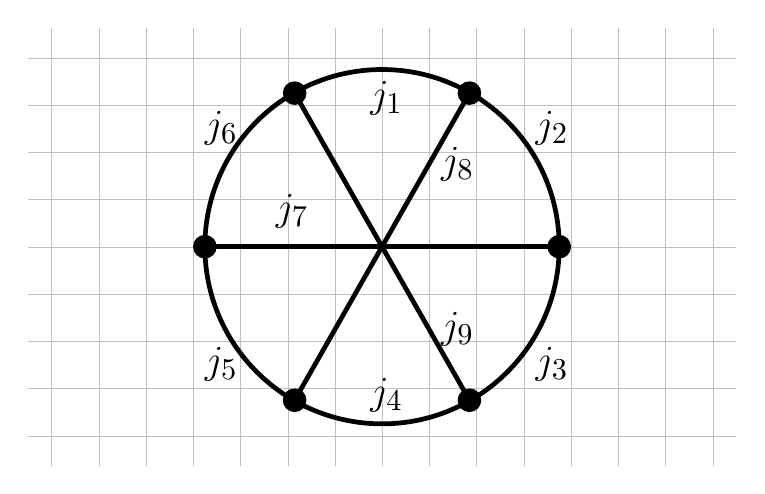
\begin{tikzpicture}[ thick,scale=3]
	
	% (VP_ml-B)
	\draw[gray!50,line width=0.01mm,step=0.2] (-0.5,0.073) grid (2.5, 1.927);
	\draw[line width=0.6mm] (1,1) circle (.75);
\fill (0.25,1) circle (0.05);
\fill (1.75,1) circle (0.05);
\fill (0.63,1.65) circle (0.05);
\fill (0.63,0.35) circle (0.05);
\fill (1.37,1.65) circle (0.05);
\fill (1.37,0.35) circle (0.05);
\draw[line width=0.6mm] (0.25,1) -- (1.75,1);
\draw[line width=0.6mm](0.63,1.65) -- (1.37,0.35);
\draw[line width=0.6mm] (0.63,0.35) -- (1.37,1.65);
	\node at (1,1.63) {\fontsize{15pt}{0} $j_1$};
	\node at (1.7,1.5) {\fontsize{15pt}{0} $j_2$};
	\node at (1.7,0.5) {\fontsize{15pt}{0} $j_3$};
	\node at (1,0.37) {\fontsize{15pt}{0} $j_4$};
	\node at (0.3,0.5) {\fontsize{15pt}{0} $j_5$};
	\node at (0.3,1.5) {\fontsize{15pt}{0} $j_6$};
	\node at (0.6,1.15) {\fontsize{15pt}{0} $j_7$};
	\node at (1.3,1.35) {\fontsize{15pt}{0} $j_8$};
	\node at (1.3,0.65) {\fontsize{15pt}{0} $j_9$};

\end{tikzpicture}

\end{document}